\section{System's Perspective}
\label{sec:systems_perspective}

\subsection{Overview}
\label{subsec:systems_perspective_overview}
The initial project was a full stack Flask application written in Bash and Python2 with an SQLite database. 
This implementation (henceforth referenced as TBD-MiniTwit) included refactoring the initial project to the following containerized microservices:
\begin{itemize}
    \item C\# backend using the ASP.NET web framework and EF Core ORM
    \item ReactJS SPA frontend
    \item PostgreSQL database
\end{itemize}
upon which a monitoring and (temporarily) a logging stack were added to be served as a containerized application behind a load-balancer on a managed Kubernetes cluster.

\subsection{System Design}
\label{subsec:system_design}
% - Design of your ITU-MiniTwit systems
The heart of TBD-MiniTwit is the C\# backend.
It contains all our business logic and provides two open APIs, an Object-Relational Mapping to our database and exposes application-specific metrics for Prometheus. \\
CLASS DIAGRAMS FOR BACKEND \\
STATE MACHINE DIAGRAM FOR LOGIN \\
%This will be the module viewpoint

\begin {figure}[H]
    \centering
    \includegraphics[draft]{foo}
    \caption{Package overview diagram fro MiniTwit-TBD}
    \label{fig:legacyDeploy}
\end{figure}

\begin {figure}[H]
    \centering
    \includegraphics[draft]{foo}
    \caption{Decomposition of x package of the POS system}
    \label{fig:legacyDeploy}
\end{figure}



\begin {figure}[H]
    \centering
    \includegraphics[draft]{foo}
    \caption{C&C overview of MiniTwit-TBD}
    \label{fig:legacyDeploy}
\end{figure}


\subsection{System Architecture}
\label{subsec:system_architecture}
% - Architecture of your ITU-MiniTwit systems
% - All dependencies of your ITU-MiniTwit systems on all levels of abstraction and development stages.
% - That is, list and briefly describe all technologies and tools you applied and depend on.
This implementation follows the \textbf{Microservice Architecture Pattern} \\
EXPLAIN THE PATTERN \\
CREATE DIAGRAMS \\
\begin {figure}[H]
    \centering
    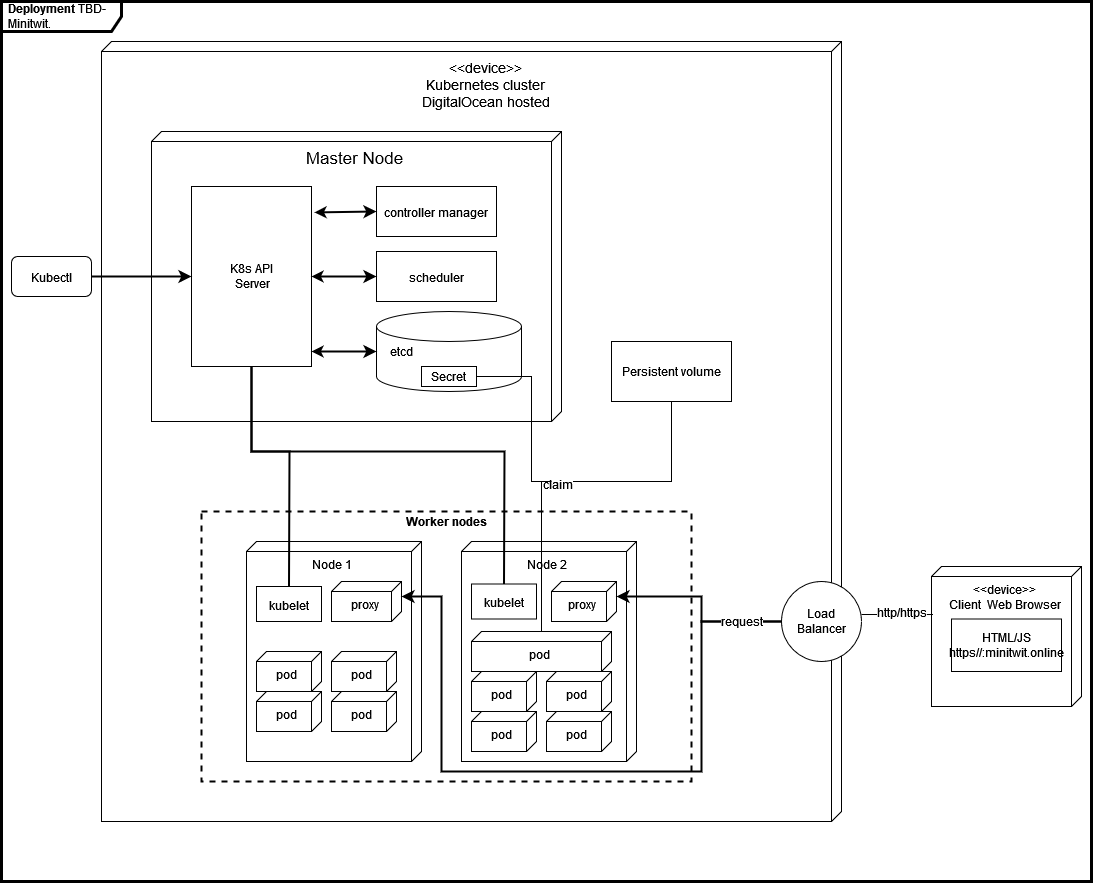
\includegraphics[scale=0.45]{images/DevopsDiagrams-Deployment k8s.drawio.png}
    \caption{TBD-MiniTwit deployment diagram}
    \label{fig:figDeploy}
\end{figure}
\begin {figure}[H]
    \centering
    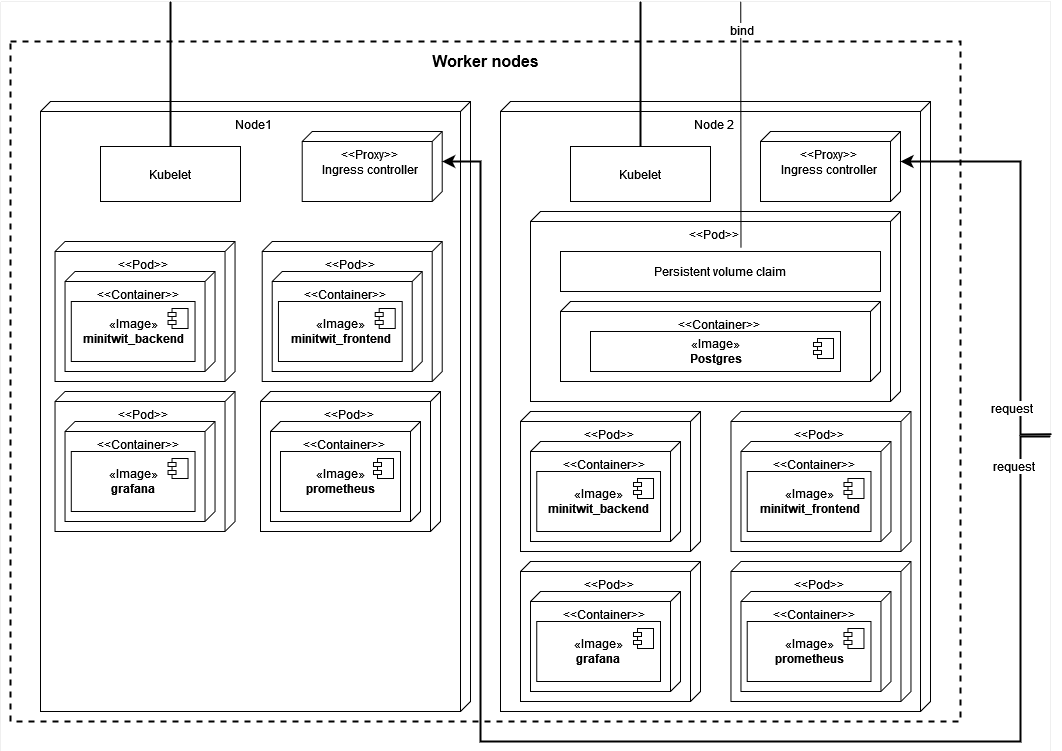
\includegraphics[scale=0.45]{images/DevopsDiagrams-Deployment worker nodes.drawio(2).png}
    \caption{TBD-MiniTwit deployment diagram. Worker nodes.}
    \label{fig:figDeployWorker}
\end{figure}

%Components and connectors view
% Allocation view.


\subsection{Subsystem Interactions}
\label{subsec:subsystem_interactions}
% - Important interactions of subsystems
\begin{table}[h!]
    \centering
    \begin{tabular}{|c|} \hline
         Prometheus \\ \hline
         MinitwitAPI \\ \hline
         LoadBalancer \\ \hline
    \end{tabular}
    \caption{Network interfaces}
    \label{tab:my_label}
\end{table}

\subsection{System state}
\label{subsec:system_state}
% - Describe the current state of your systems, for example using results of static analysis and quality assessment systems.
% Wait until after cleanup when frontend is merged.
\hyperref[app:codeAnal]{Code analysis dashboards}
To be able to argue about the quality of our code, we have enhanced our CI pipeline with static code analysis tools. These analyse and rate the TBD-MiniTwit in accordance with their own definition of code quality. According to the \hyperref[fig:hubStatus]{Better Code Hub quality status} our codebase is in compliance with 9 of 10 measures for quality, while failing on code duplication. The reason for this is, that the MiniTwit system supports both a simulator api and an api for the frontend. When refactoring infrastructure code for the frontend api, we kept the infrastructure for the simulator resulting in code duplication.
Sonarcloud suggests that we have a technical debt of 55min, all of which is from the Simulation Controller and it´s infrastructure class. It also located 8 code smells, but still gives the main branch an grade of A. See \hyperref[fig:cloudMaintainability]{sonarcloud maintainability scores} 



\subsection{License Compatibility}
\label{subsec:license_compatability}
% - Finally, describe briefly, if the license that you have chosen for your project is actually compatible with the licenses of all your direct dependencies.
%this is only a draft - the file from scancode is quite big, so still missing some parts..
The initial license chosen was MIT, which means everyone can use and modify the code freely.
However, when we used a tool called \textit{ScanCode} (\footnote{Scancode toolkit documentation\cite{Scancode}}) to determine if our chosen license would clash with a license in the imports we use by scanning the files in the project, we discovered that some of our imports used Apache License 2.0 and BSD-3-Clause, meaning we had to change license. Some imports used all three licenses mentioned above. The tool has briefly been mentioned throughout the course.
The new license is Apache 2.0 as a result of running \textit{ScanCode} to have a license that is compatible with our imports. The scan seemed to fail on some licenses as it stated them as \textit{Unknown license}, however, since the other licenses encountered are the three mentioned previously, then it is likely not to be a problem.
%Idk if you want to check for yourself if multiple licenses are used in the same file.. but an example is The pack in line 50432-51470 in result.json, which is quite a big file.

%NEEDS REWRITE - turns out the imports we use in the code only uses MIT and Apache 2.0... seems like the other licenses are the imports' dependencies' licenses - the imports we use licenses is below.
%React.router = mit license
%react-router-dom = mit license
%prop-types = mit license
%@mui/material = mit license
%markdown-to-jsx = mit license
%react = mit license
%react-router = mit license
%yup = mit license
%formik = Apache license 2.0

% A description and illustration of the:
% - Double check that for all the weekly tasks (those listed in the schedule) you include the corresponding information.